\begin{figure}[htp]
\centering
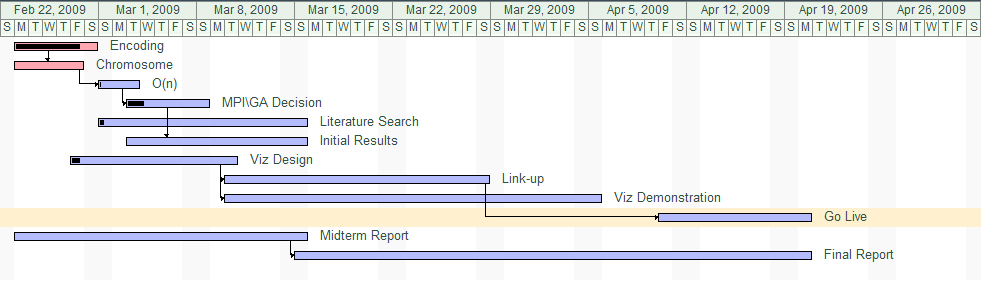
\includegraphics[width=1\textwidth]{images/gantt.png}
\caption{Project timeline of major milestones}\label{fig:gantt}
\end{figure}
Figure \ref{fig:gantt} shows a detailed timeline for the completion of the project. The major milestones for all aspects of the project present, including necessary work for the creation of an optimization scheme to seach for universal turing machines as well as the creation of a web based visualization tool to faciliate the examination of the project results. The key to the task names used in Figure \ref{fig:gantt} is presented below: 
\begin{itemize}
	\item {\bf Encoding}:	Definition of the encoding method for Turing Machines completed
	\item {\bf Chromosome}: Implementation of the chromosome class for the AI4R Genetic Algorithm package completed.
	\item {\bf O(n)}:	Computational cost for fitness evaluation of a Turing Machine is determined.
	\item {\bf MPI/GA Decision}:	Decision made regarding necessity of use for MPI along with AI4R Genetic Algorithm to reduce computation time.
	\item {\bf Litearture Search}: Literature search to generate a list of known UTM  
	\item {\bf Initial Results}: Initial Turing Machine Optimization run completed. Data analyzed to ensure the viability of optimzation scheme
	\item {\bf Viz Design}: Visualization web-app design complete
	\item {\bf Link-up}: Link between genetic algorithm generation data and visualization database completed.
	\item {\bf Viz Demonstration}: Ruby on Rails visualization application implementation completed.
	\item {\bf Go Live}: Ruby on Rails visualization application goes live with link to genetic algorithm running perpetually.
	\item {\bf Midterm Report}: Midterm Report Delivery
	\item {\bf Final Report}: Final Report Delivery
	\item {\bf Presentation}:	Final Presentation
\end{itemize}